\documentclass[a4paper,12pt]{article} % тип документа

% report, book



%  Русский язык

\usepackage[T2A]{fontenc}			% кодировка
\usepackage[utf8]{inputenc}			% кодировка исходного текста
\usepackage[english,russian]{babel}	% локализация и переносы
\usepackage{graphicx}
\graphicspath{{./}}
\DeclareGraphicsExtensions{.png,.jpg}


% Математика
\usepackage{amsmath,amsfonts,amssymb,amsthm,mathtools} 


\usepackage{wasysym}

%Заговолок
\author{Бредихин Александр}
\title{Домашняя работа №7}



\begin{document} % начало документа
\maketitle
\subsection*{Задача 1}
\textit{Задача: реализуйте стек с помощью двух очередей.}\\

По определению стек -- достаём первым элемент тот, который последний положили. Очередь -- FIFO: достаём первым тот, который первым положили. Рассмотрим два способа реализовать стек с помощью двух очередей:
\begin{itemize}
\item[1) ] дорогостоящая push опреация\\ 
Одну из очередей всегда держим пустой. В другой элементы будут лежать в обратном порядке их поступления для этого при добавлении нового элемента делаем следующие операции: кладём новый элемент в пустую очередь, затем из другой <<вытаскиваем>> элементы и кладём в первую очередь. Всю полученную очередь перекладываем, чтобы она стала пустой (или просто переименовывываем названия). Заметим, что при такой операции, последний поступивший элемент будет первым в очереди. Удаление элемента это извлечение первого элемента из непустой очереди (или ошибка, если обе очереди пусты).\\
Пример работы при добавлении 2, в наш стек, в котором уже есть элемент 1. В результате в одной из очереди элементы располагаются в обратном порядке, а другая очередь остаётся пустой.
\begin{center}
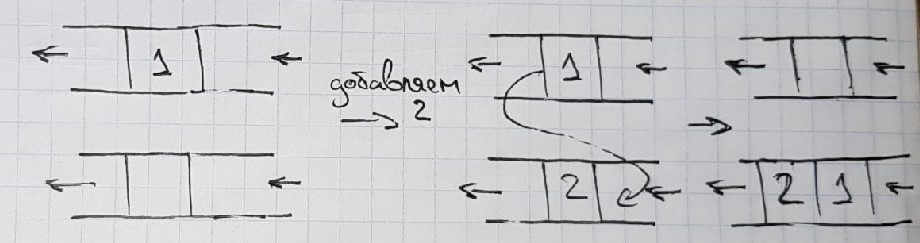
\includegraphics[width=0.7\textwidth]{ex_1}
\end{center} 

\item[2) ] дорогостоящая pop операция\\
Также оставляем одну очередь пустой, в другую кладём элементы в порядке поступления. При операции извлечения достаём из очереди все элементы до предпоследнего включительно и кладём их в пустую очередь. Последний элемент остаётся один, извлекаем его. В итоге достаём тот элемент, который последним положили, следовательно, стек.
\end{itemize}

Заметим, что в первом случае при операции push мы перекладываем все элементы из одной очереди в другую: $ \mathcal{O}(n) $ где $ n $ -- количество элементов в стеке, но операци pop занимет $ \mathcal{O}(1)$. Во втором же, наоборот, операция pop делается за $ \mathcal{O}(n) $, а push за $ \mathcal{O}(1)$\\ (можно подсчитать амортизационную сложность и скорее всего она будет равняться $ \mathcal{O}(1)$ для обоих операций).

\subsection*{Задача 2}
\textit{Задача: опишите способ хранения почти-полного троичного дерева в массиве. Как по номеру клетки родителя вычислить номера детей? Как по номеру ребёнка вычислить номер родителя?}\\

Дерево будем хранить аналогично почти-полному бинарному дереву. То есть нумерация элементов начинается с 1 и располагаем элементы, которые находятся на одном уровне подряд в массив слева направо спускаясь по уровням вниз.\\
Пусть $ k $ номер ячейки родителя, тогда его дети будут с номерами: $ 3k - 1, \quad 3k, \quad 3k+1 $. Покажем это: пусть родитель располагается на уровне $ h $ и на $ n $ом месте слева на своём уровне. Тогда до него количество элементов в массиве равно (то есть его номер ячейки в массиве):
$$
k = 1+3+ \cdots + 3^{h-1} + n
$$
Аналогично считаем позицию для его детей и выражаем её через $ k $. Для самого левого ребёнка:
$$ 
1 + 3 + \cdots + 3^h + 3(n-1) + 1 = (3 + 9 + \cdots + 3^h) +2 - 3 = 3k - 1
$$
для центрального и правого ребёнка формулы будут иметь вид:
$$ 
1 + 3 + \cdots + 3^h + 3(n-1) + 2 = 3k - \text{центральный ребёнок}
$$
$$
1 + 3 + \cdots + 3^h + 3(n-1) + 3 = 3k + 1 - \text{правый ребёнок}
$$
Следовательно, дети имеют номера:  $ 3k - 1, \quad 3k, \quad 3k+1 $.\\

Пусть $ m $ -- номер ребёнка, тогда его родитель имеет номер: $ \left[\frac{m}{3} \right] $, где $ \left[\frac{m}{3} \right] $ -- округление до ближайшего целого при делении на 3. Это напрямую следует из формул, которые мы получили выше.



\subsection*{Задача 3}
\textit{Задача: Докажите, что если в бинарном дереве поиска у элемента $x$ нет правого ребёнка и у $x$ есть следующий за ним в порядке возрастания элемент~$y$, то $y$ является самым нижним предком $x$, чей левый дочерний узел так же является предком $x$ или самим~$x$.}\\

Сначала покажем, что $ y $ является предком $ x $ а затем, что самым нижнем.\\
От противного: пусть $ y $ не является предком $ x $, тогда существует узел $ a $, который является предком и для $ x $ и для $ y $ при этом эти два элемента лежат в разных поддеревьях узла $ a $: так как $ x < y $, то $ x $ лежит в левом поддереве, а $ y $ в правом. Так как это бинарное дерево поиска, то по его определению верно такое неравенство: $ x < a < y $ (б.о.о считаем, что элементы в узлах различны). Получили противоречие, с тем, что $ y $ следующий в порядке возрастания элемент за $ x $ (есть ещё $ a $), следовательно, $ y $ -- предок $ x $.\\

Докажем, что $ y $ -- самый нижний предок (так как $ x < y $, то $ x $ будет располагаться в левом поддереве $ y $). Снова от противного, пусть это не так: то есть у $ y $ существует левый дочерний узел $ a $, который является предком $ x $ и $ a  != x, y \quad $, тогда по определению бинарного дерева поиска получаем, что $ x < a < y $ -- противоречие. Следовательно, $ y $ -- самый нижний предок $x$, чей левый дочерний узел так же является предком $x$ или самим~$x$.


\subsection*{Задача 4}
\textit{Задача: покажите, что если вершина~$b$ в бинарном дереве поиска имеет две дочерние вершины, то последующая за ней вершина~$c$ не имеет левой дочерней вершины, а предшествующая ей вершина~$a$~"--- правой. Под предшествующей и последующей вершиной понимается, что $a.key \leq b.key \leq c.key$ и в дереве поиска нет ключей в промежутках $(a.key,b.key)$ и $(b.key,c.key)$.}\\

Докажем для вершины $ c $, что она не будет иметь левой дочерней вершины, для вершины $ a $ аналогично. Доказываем от противного: пусть у вершины $ c $ есть левый ребёнок, обозначим его $ k $. Возможны 2 случая:
\begin{itemize}
\item[1) ] Пусть $ k.key > b.key $. Из условия в дереве поиска нет ключей в промежутке $(b.key,c.key)$, следовательно, будет выполняться неравенство, что $ b.key < c.key < k.key $, а это невозможно так как $ k $ -- левый ребёнок для $ c $, значит, $ k.key < c.key $ (по определению бинарного дерева). Получили противоречие.
\item[2) ] Пусть $ k.key < b.key $. Заметим, что в этом случае $ c $ не может быть в левом поддереве $ b $, так как нарушится условие, что $ c.key > b.key $ (если бы $ c.key = b.key $, то тогда по определению бинарного дерева выполнялось бы соотношение, что $ с.key \leq k.key \leq b.key $, но в промежутке $(b.key,c.key)$ нет ключей).\\
Также $ c $ не может находиться в правом поддереве $ b $, так как тогда $ b.key < k.key $, что разбиралось уже в 1ом случае.\\
Получается, что $ c $ может быть либо предком вершины $ b $, либо будет существовать вершина $ m $ -- предок и $ b $ и $ c $, такая что $ b $ и $ c, k $ лежат в разных поддеревьях. Притом $ b $ в левом, иначе не выполнится условие, что $ b.key \leq c.key $. \\
Для первого варианта, если $ c $ -- потомок, то рассмотрим правого ребёнка $ b $ обозначим его за $ p $. Из определения бинарного дерева будет следовать, что $ b.key \leq p.key \leq c.key $, получили противоречие, что в нашем дереве поиска нет ключей в промежутке $(b.key,c.key)$.\\
Для второго получим это же противоречие: $ b.key \leq m.key \leq c.key $. 
\end{itemize}
Рассмотрели тут все случаи и везде пришли к противоречию, следовательно изначальное утверждение, что у вершины $ c $ есть левый ребёнок - неверно.


\subsection*{Задача 5}
\textit{Задача:} известно, что в структуре данных потребуется хранить $k$-элементное подмножество $A$ $n$-элементного множества. После того как в структуру данных будет загружено множество $A$, с помощью неё будет нужно проверить принадлежит ли $A$ элемент $x$. Для этого можно совершить не более $t$ запросов к структуре: каждый запрос $q$ представляет собой конечную строку битов, ответ на каждый запрос~"--- один бит. 

Структура данных представляет собой таблицу с двумя столбцами: первый столбец состоит из всевозможных запросов $q$ (известных заранее), а правый из битов-ответов на запрос -- правый столбец формируется после загрузки в структуру множества $A$.  Пусть $s(n,k,t)$ -- минимальное количество строк в такой таблице которое достаточно отвести под такую структуру данных.\\
Чему равно $s(n,k,1)$?\\


Так как $ t = 1 $, то мы должны за одно обращение к структуре понять принадлежит ли $ x $ A или нет. Пусть таблица будет с вопросами вида принадлежит ли элемент множеству $ A $ или нет и так для каждого элемента $ n $го множества, то есть $ n $ строк запросов.
\\ Почему меньше, чем $ n $ нельзя? Тогда для двух различных чисел будет один и тот же вопрос, на который можно ответить, только 2мя способами (по условию задачи ответ - 1 бит). А вариантов 4: оба принадлежат, одно принадлежит другое нет, оба не принадлежат. То есть не сможем однозначно установить вхождение в $ A $.



\subsection*{Задача 6}
\textit{Задача: К серверу приходят одновременно $n$ клиентов. Для клиента $i$ известно время его обслуживания~$t_i$. Время ожидания клиента определяется как сумма времени обслуживания всех предыдущих клиентов и времени обслуживания его самого. К примеру, если обслуживает клиентов в порядке номеров, то время ожидания клиента~$i$ будет равно $\sum\limits_{j=1}^{i} t_j$. Постройте эффективный алгоритм, находящий последовательность обслуживания клиентов с минимальным суммарным временем ожидания клиентов.}\\

Заметим, что минимальное время ожидание для каждого клиента -- это время обслуживание его самого. Докажем, что выгоднее (тогда суммарное время ожидание будет минимальным) обслуживать клиентов, на которых уходит меньше времени.\\
От противного: рассмотрим двух клиентов время обслуживания которых: $ t_1 $ и $ t_2 $ при этом $ t_2 > t_1 $, и обслуживается сначала 2ой клиент, а затем 1ый.\\ Заметим, что если мы поменяем их местами, то время ожидания клиентов до 2го и после 1го не изменятся (так как для тех которые перед ними не важно, что происходит после них, а те которые за ними все равно будут ждать обоих). Время ожидания 1го уменьшится на $ t_2 $ а 2го увеличится на $ t_1 $.\\ Получается суммарное ожидание всех клиентов уменьшится на $ t_1 - t_2 $, следовательно, выгоднее обслуживать клиентов с меньшим временем.\\
Из этих рассуждений следует, что мы отсортируем клиентов по возрастанию времени ожидания это и задаст оптимальный порядок их обслуживания. Суммарное время ожидания всех клиентов может быть найдено по следующей формуле:
$$
t_1 + (t_1 + t_2) + \ldots + (t_1 + t_2 + \ldots + t_n) = t_1n + t_2(n-1) + \ldots + t_n
$$
где $ t_1 $ -- время обслуживания клиента, который пошёл первым (с наименьшим временем) и так далее. \\
Сложность выполнения алгоритма -- $ \mathcal{O}(n\log(n))$ (сортируем клиентов по возрастанию времени их обслуживания).


\begin{center}
\begin{Large}
Из восьмой домашней работы
\end{Large}
\end{center} 


\subsection*{Задача 4}
Задача: опишите реализацию структуры данных <<очередь с приоритетами>> (из классного листка) со следующими стоимостями операций 

\begin{itemize}
	\item \texttt{insert}~"--- $O(1)$,
		\item \texttt{extract\_max}~"--- $O(n)$, 	\item \texttt{set\_priority}~"--- $O(1)$. 
\end{itemize}
При этом известно, что все ключи~"--- уникальные числа в диапазоне от $1$ до $n$.\\

Используем обычный массив. Ключами нашей очереди с приоритететом являются индексы массива, а их приоритетом значение в массиве с этими индексами. Это можно сделать, так как все индексы уникальны и лежат подояд в диапозоне от $1$ до $n$ (как индесы массива).\\
Тогда стоимость нужных нам операций будет равна:
\begin{itemize}
\item[1) ] Вставка за $O(1)$ -- добавляем элемент в конец массива, зная его размер (так как все ключи разные и идут подряд, то новый элемент всегда будет вставать на последнее место) -- константа по времени.
\item[2) ] \texttt{extract\_max}~"--- $O(n)$: проходим циклом по массиву и находим ключ с максимальным приоритетом, а затем выводим этот ключ и его приоритет.
\item[3) ] Установление приоритета по ключу $ k $ -- $O(1)$. Так как меняем значение в массиве по индексу $ k $
\end{itemize}



\subsection*{Задача 5}
\textit{Задача:} постройте оптимальный алгоритм, который находит минимальный элемент в куче на максимум.\\

Докажите, что ваш алгоритм оптимальный: если ваш алгоритм работает за время $O(f(n))$, то любой алгоритм работает за время $\Omega(f(n))$. Считайте, что алгоритм не знает элементы заранее, куча хранится в памяти как массив $a$ и алгоритм может за один запрос $i$ узнать элемент $a[i]$.\\

По определению кучи на максимум: каждый ребёнок вершины меньше, чем она сама, поэтому минимальный элемент должен содержаться в одном из листов (иначе уже будет какая-то вершина, которая меньше его). Листом считаем и те вершины, уровень которых на 1 меньше (если бинарное дерево неполное), то есть все вершины у которых нет листьев.\\
Из теории графов следует, что в почти-полном бинарном дереве не может быть больше $ \left[ \frac{n}{2} \right] $ листьев. При этом в массиве, в котором хранится куча, они идут подряд (начиная с $ \left[ \frac{n}{2} \right] $ до конца). Наш алгоритм находит из них минимальное, оно и будет минимальным в куче.\\
Так как в худшем случае (полное бинарное дерево) нужно проверить $ \left[ \frac{n}{2} \right] $ листьев, то сложность алгоритма $ O(n) $. \\

Почему быстрее нельзя? Докажем, что необходимо проверить все листья, чтобы найти минимальный элемент в куче. От противного, пусть это не так и существует алгоритм в котором какой-то из листьев мы не смотрим. Запустим этот алгоритм и найдём минимальное число. Поставим в лист, который мы не просматриваем число меньше минимального, куча при этом никак не изменится (по определению кучи), соответственно алгоритм сделает все те же шаги и вернёт то же число. Но оно уже не минимальное. Получили, что алгоритм некорректный, следовательно необходимо просмотреть все листья, которых в худшем случае $ \left[ \frac{n}{2} \right] $, поэтому быстрее, чем за $ O(n) $ решить нельзя. 


\subsection*{Задача 6}
Задача: дан массив из $n+1$ элемента, который содержит элементы от $1$ до $n$ и известно, что каждое число от $1$ до $n$ встречается хотя бы один раз. 
\begin{itemize}
\item[1) ] Докажите, что какое-то число от $1$ до $n$ встречается два раза.
\item[2) ] Предложите алгоритм, который находит дубликат за $O(n)$.
\item[3) ] Предложите алгоритм, который находит дубликат за $O(n)$ и $O(1)$ дополнительной памяти.
\end{itemize}

$1)$ Это следует из признака Дирихле: так как всего $ n $ ящиков (возможные числа) и $ n+1 $ элементов (в каждом элементе массива должно быть число), следовательно хотя бы одно из чисел встретится дважды.\\ Заметим, что будет только одно повторение, так как все элементы от $1$ до $n$ встречается хотя бы один раз. \\

$ 2) $ Создадим массив длинной $ n $ сначала заполненный нулями, индекс массива будет означать само число, соответствующие значение этому индексу -- количество раз, которое этот элемент встречался в исходном массиве.\\
Алгоритм: пробегаемся по исхожному массиву и прибавляем 1 элементу нового массива с индексом встретившегося числа. Затем пробегаем по новому массиву и выводим индекс, где значение равно 2 (индексация нового массива начинается с 1).\\
Корректность алгоритма следует из рассуждения в пункте 1). Сложность: по времени и по памяти  $O(n)$, так как пробегаемся 2 раза по массивам сначала длины $ n+1 $, затем $ n $ и создаём новый массив длины $ n $.\\

$ 3) $ Теперь будем использовать $O(1)$ дополнительной памяти: заведём переменную $ sum $. Пройдёмся циклом по исходному массиву и будем прибавлять значение каждого элемента к этой переменной, то есть в ней будет находиться сумма всего массива. В пукте 1) заметили, что все элементы встречаются хотя бы один раз. Сумма элементов от $1$ до $n$ равняется $S = \frac{n(n+1)}{2} $. Поэтому вычитая из $ sum - S $, получим элемент, который встретился дважды.\\
Нахождение суммы всего массива -- $O(n)$. Из дополнительной памяти используем только переменную $ sum $ -- $O(1)$.

\subsection*{Задача 7}
\textit{Задача: постройте алгоритм, который получив на вход числовой массив выводит количество его подмассивов (непрерывных подпоследовтаельностей), в которых все элементы различны.}

Сначала приведём пример того, что хотим реализовать. Пусть на вход подали массив 1 2 3 2 5, тогда алгоритм должен подсчитать следующие подмассивы:\\
1 \\ 1 2\\ 1 2 3\\ 2 \\ 2 3 \\ 3 \\ 3 2 \\ 3 2 5 \\ 2 5 \\ 5\\
Для реализации этого создадим словарь $ s $, переменную $ res $ в которой будем хранить количество подмасивов и $ start $ -- указатель откуда начинаем считать.\\
1) Идём по нашему массиву и если считанного элемента нет в словаре, то добавляем его туда (индекс -- значение, значение -- индекс элемента). Также делаем операцию $ res ++ $\\
2) Если элемент есть в массиве и $ i \geq start $, то $ start++ $ и все значения словаря, которые больше, чем $ start + 1 $, делаем NULL.\\
3) Если считанный элемент уже есть в массиве и $ i < stat$, то $s[a[i]] = i$ и $ res++ $.\\
4) Если мы дошли до последнего элемента и для него не выполняется пукт 2), то $res += \frac{(n -start - 1) \cdot (n-start)}{2}$ (индексация начинается с 1).\\
То есть если простыми словами, то мы идём <<рамкой>> по нашему массиву и запоминает, где последний раз видел элемент. Если элемент ещё не встречался, то подмассив уникален и мы его считаем. Если элемент уже встречался до $ start$, и его позиция в словаре равна NULL, то подмассив остаётся со $ start $ до $ i $ уникальным и мы запоминаем его новое положение в словаре и снова увеличиваем счётчик. Если мы встречаем элемент после позиции старт, то со $ start $ до $ i $ подмассив не уникален и мы двигаем положение $ start $ на 1. 4ый пункт нужен для выведения подмассивов, которые не учтутся этим алгоритмом, так как мы дойдём до последнего элемента (корректность следует из описания алгоритма).\\
Сложность: в худшем случае будем кадый раз бегать по словарю и ставить NULL. Длина массива $ n $ и длина словаря может достигать $ n $, поэтому сложность оценивается, как $ O(n^2) $.

\subsection*{Задача 8}
Задача: cтруктура данных <<таблица>> представляет собой числовую матрицу размера $m\times n$ (двумерный массив), элементы которой в каждой строке и каждом столбце отсортированы по возрастанию. В случае, если в таблице меньше $mn$ элементов, в незаполненных клетках написано $\infty$. \\

1)  Постройте алгоритм, который проверяет находит элемент $x$ в  частично заполненную таблицу за $O(m+n)$ или проверяет, что такого элемента в таблице нет.\\

2) Постройте алгоритм, вставляющий новый элемент в частично заполненную таблицу за $O(m+n)$.\\

1) Начнём с верхней правой ячейки и будем делать следующие: пока элемент слева больше $ x $ (элемент, котрый мы хотим проверить на вхождение), двигаемся влево. Если это условие не выполнено, то смещаемся на 1 строку вниз и снова проверяем первое условие. Заканчиваем эти действия, если какой-то из элементов таблицы равен $ x $ или если больше не можем делать шагов (то есть дошли до самой нижней строчки и слева по строке элемент меньше), тогда $ x $ в таблице нет.\\

Корректность: заметим, что переходя влево на одну ячейку мы проверяем весь столбец, так как $ A > x $ и все элементы выше $ A $ больше его (так как столбец отсортирован по возрастанию). Также переходя на строку вниз мы проверяем всю строку, так как $ x > B $ и все элементы левее $ B $ в этой строке меньше его (так как строка отсортирована). Получается, дойдя до последней строки (когда мы уже не сможем делать шаги) мы проверим всю таблицу. Если элемента $ x $ не было найдено, то его точно нет в таблице.\\

Сложность: в худшем случае $ x $ будет находится в нижнем левом углу, до него нужно сместиться на $ m $ строк вниз и на $ n $ столбцов влево. Каждое смещение делается с операцией сравнения, которая стоит $ O(1) $, поэтому сложность $ O(m+n) $.\\

2) Для добавления элемента $ a $ делуем следующие шаги: начинаем с правого нижнего угла таблицы и пока $ max(x,y) > a $, где $ x $ -- элемент который ниже текущей позиции, $ y $ -- правее текущей позиции, меняем $ max(x, y) $ и $ a $. Затем, когда это невозможно, то есть когда цикл <<while>> завершится ставим элемент $ a $ в текущее место. (Возникают некоторые тонкости, как начать алгоритм. Не учитывать $ \infty $ при начальном сравнении и т.д.)\\

Корректность: нужно проверить, что при таких действиях не нарушается отсортированность по строкам и по столбцам (начинаем с самого большого элемента, так как все строки и столбцы отсортированы по возрастанию). Заметим, что вправо и вверх ставим элемент, который больше, чем $ a $, когда не сможем это сделать, то все элементы выше текущего положения и левее будут меньше $ a $ (так как тогда $ a > max(x,y) $ и все элементы ниже $ x $ и левее $ y $ меньше их). То есть в них отсортированность не нарушилась, также так как мы меняем с $ max(x,y) $ не нарушается и в верхней части таблицы (и по строке и по столбцу).\\

Сложность: в худшем случае элемент $ a $ нужно будет поставить на левый верхний угол, то есть сложность, как и в предыдущем пункте $ O(n+m) $.



\end{document} % конец документа